
Software engineering and software architecture is a very complex matter, and the natural way to deal with uncertainties is to insure yourself against potential risks. We do it all the time with life insurance, health insurance, and car insurance. Yet when it comes to software development, we tend to forget about all the safety precautions and just hope for an optimistic outcome.

Knowing that things not only may but will go wrong, it is unbelievable that the topic of testing software is still a controversial one. Whether it's from having a lack of skill or from a lack of budget, there are still projects that lack even some of the most basic tests. And when the client decides to change the requirements, a simple correction may result in endless reworks and firefights.

The time that's saved from not implementing proper testing is lost when the first rework happens. If you think this rework will not happen very soon, you are most probably very mistaken. In the agile environment we live in nowadays, reworks are a part of our daily life. Our knowledge about the world and our customers' changes means that the requirements change, and with that comes making changes to our code.

Therefore, testing's main purpose is to protect your precious time later in the project. Sure, it's an investment early on when you have to implement various tests instead of focusing solely on the features, but it's an investment you won't regret. Like an insurance policy, testing takes a little from your budget when things go according to plan, but when things go bad, you'll get a generous payout.


\subsubsubsection{8.2.1\hspace{0.2cm}The testing pyramid}

There are different types of testing you may encounter when designing or implementing a software system. Each of the classes serves a slightly different purpose. They can be categorized as follows:

\begin{itemize}
\item 
Unit testing: Code

\item 
Integration testing: Design

\item 
System testing: Requirements

\item 
Acceptance testing (end-to-end or E2E): Client needs
\end{itemize}

This distinction is arbitrary and you may often see other layers of the pyramid, as follows:

\begin{itemize}
\item 
Unit testing

\item 
Service testing

\item 
UI testing (end-to-end or E2E)
\end{itemize}

Here, unit testing refers to the same layer as in the previous example. Service testing refers to a combination of integration testing and system testing. On the other hand, UI testing refers to acceptance testing. The following diagram shows the testing pyramid:

\begin{center}
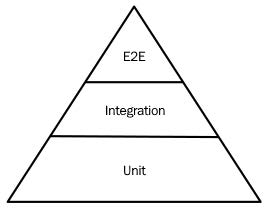
\includegraphics[width=0.9\textwidth]{content/3/chapter8/images/1.jpg}\\
Figure 8.1 – Testing pyramid
\end{center}

It's worth noting that unit tests are not only the cheapest to build but that they also execute pretty quickly and can often run in parallel. This means they make for a great continuous integration gating mechanism. Not only that, but they also often provide the best feedback about the health of your system. Higher-level tests are not only harder to write properly, but they also may be less robust. This can lead to flickering test results, with one in every few test runs failing. If the failure in the higher-level test is not correlated with any failure at the unit test level, chances are that the problem may be with the test itself and not in the system under test.

We don't want to say that the higher-level tests are entirely useless and that you should only focus on writing unit tests. That's not the case. The pyramid has its shape because there should be a solid base covered by unit tests. On that base, however, you should also have all the higher-level tests in an appropriate proportion. After all, it is not very hard to imagine a system where all the unit tests are passing, but the system itself doesn't provide any value to the customer. An extreme example would be a perfectly working backend without any user interface (be it graphical or in the form of an API) present. Sure, it passes all the unit tests, but that's no excuse!

As you may imagine, the opposite of the testing pyramid is known as an ice cone, and it is an antipattern. Violating the testing pyramid often leads to fragile code and hard to trace bugs. This makes debugging much more expensive and doesn't introduce savings in test development either.

\subsubsubsection{8.2.2\hspace{0.2cm}Non-functional testing}

What we've already covered are so-called functional tests. Their aim is to check whether the system under test fulfills the functional requirements. But there are also other types of requirements besides functional ones that we may want to control. Some of them are as follows:

\begin{itemize}
\item 
Performance: Your application may behave according to requirements in terms of functionality but still be unusable for end users due to weak performance. We will focus more on improving performance in Chapter 11, Performance.

\item 
Endurance: Even if your system can be really performant, it doesn't mean it can survive a continuously high workload. And when it does, can it survive some of the malfunctionings of the components? When we embrace the idea that every piece of software is vulnerable and may break at any given moment, we start designing systems that can be failure-resistant. This is a concept that the Erlang ecosystem embraces, but the concept itself is not limited to that environment alone. In Chapter 13, Designing Microservices, and Chapter 15, Cloud-Native Design, we will mention a bit more about designing systems that are faulttolerant and the role of chaos engineering.

\item 
Security: Nowadays, there should be no need to repeat that security is crucial. But since it still isn't treated with all the seriousness the matter requires, we will bore you with saying this yet again. Every system that is connected to the network can – and most probably will – be broken. Performing security tests early on during development gives the same benefits as other kinds of tests: you can catch problems before they are too expensive to fix.

\item 
Availability: Whereas poor performance may discourage your end users from using your product, poor availability may prevent them from even accessing said product. While availability problems may arise due to performance overload, there are also other causes of lost availability.

\item 
Integrity: Your customers' data should not only be safe from outside attackers. It should also be safe from any alterations or losses due to software malfunction. Protection against bit rot, snapshotting, and backups are ways to prevent integrity loss. By comparing the current version with previously recorded snapshots, you can make sure if the difference resulted only from the action that was taken or whether it was caused by errors.

\item 
Usability: Even a product that ticks all of the previous boxes may still be unsatisfactory for the users if it has a clunky interface and unintuitive interaction. Usability tests are mostly performed manually. It's important to perform a usability assessment each time the UI or the workflow of the system changes.
\end{itemize}

\subsubsubsection{8.2.3\hspace{0.2cm}Regression testing}

Regression tests are usually end-to-end tests that should prevent you from making the same mistake twice. When you (or your QA team or customers) discover a bug in a production system, it is not sufficient to apply a hotfix and forget all about it.

One of the things you need to do is write a regression test that should prevent the same error from ever entering the production system again. Good regression tests can even prevent the same class of errors from entering production. After all, once you know what you did wrong, you can imagine other ways to mess things up. Another thing you can do is perform root cause analysis.

\subsubsubsection{8.2.4\hspace{0.2cm}Root cause analysis}

Root cause analysis is a process that helps you uncover what the original source of the problem was, not only its manifestation. The most common way to perform root cause analysis is to use the method of 5 Whys, which was made famous by the Toyota company. This method consists of peeling off all the superficial layers of the problem's manifestation to uncover the root cause hidden underneath. You do this y asking "why" at each layer until you find the root cause you are looking for.

Let's look at an example of this method in action.

The problem: We didn't get payments for some of the transactions:

\begin{enumerate}
\item 
Why? The system didn't send the appropriate emails to the customers.

\item 
Why? The email sending system doesn't support special characters in customers' names.

\item 
Why? The email sending system wasn't tested properly.

\item 
Why? There was no time for proper testing due to a need to develop new features.

\item 
Why? Our time estimates for the features were incorrect.
\end{enumerate}

In this example, the problem with time estimates may be the root cause of the bug that was found in the production system. But it may as well be another layer to peel. The framework gives you a heuristic that should work most of the time, but if you don't feel entirely sure that what you got is what you are looking for, you can keep on peeling additional layers until you find what caused all the trouble.

Given that many bugs result from the exact same and often repeatable root causes, finding the root cause is extremely beneficial because you can protect yourself from making the same mistake in the future on several different levels. This is the principle of defense in depth when it's applied to software testing and problem-solving.

\subsubsubsection{8.2.5\hspace{0.2cm}The groundwork for further improvement}

Having your code tested protects you from making accidental errors. But it also opens up different possibilities. When your code is covered by test cases, you don't have to fear refactoring. Refactoring is the process of transforming code that does its job into code that is functionally similar, except it has better internal organization. You may be wondering why you need to change the code's organization. There are several reasons for this.

First of all, your code may no longer be readable, which means every modification takes too much time. Second, fixing a bug you are about to fix will make some other features behave incorrectly as the code gathered too many workarounds and special cases over time. Both of those reasons can be summed up as productivity improvements. They will make maintenance cheaper in the long run.

But apart from productivity, you may also want to improve performance. This can mean either runtime performance (how the application behaves in production) or compile-time performance (which is basically another form of productivity improvement).

You can refactor for runtime performance by replacing the current suboptimal algorithms with more efficient ones or by changing the data structures that are used through the module you are refactoring.

Refactoring for compile-time performance usually consists of moving parts of code to different compilation units, reorganizing headers, or reducing dependencies.

No matter what your end goal is, refactoring is generally a risky business. You take something that mostly works correctly and can end up either with a better version or a worse one. How would you know which case is yours? Here, testing comes to the rescue.

If the current feature set is thoroughly covered and you want to fix the recently uncovered bug, all you need to do is add another test case that will fail at that time. The moment your entire test suite starts passing again means your refactoring efforts were successful.

The worst-case scenario is that you have to abort the refactoring process in case you cannot satisfy all the test cases in a specified timeframe. You would undertake a similar procedure if you wanted to improve performance, but instead of unit tests (or end-to-end tests), you would focus on performance testing.

With the recent rise of automated tools that aid in refactoring (such as ReSharper C++: \url{https://www.jetbrains.com/resharper-cpp/features/ReSharper C++}) and code maintenance, you can even go as far as outsourcing a part of coding solely to the external software services. Services such as Renovate (\url{https://renovatebot.com/}), Dependabot (\url{https://dependabot.com}), and Greenkeeper (\url{https://greenkeeper.io/}) may soon support C++ dependencies. Having solid test coverage will let you use them without the fear of breaking your application during dependency updates.

Since keeping your dependencies up to date in terms of security vulnerabilities is something you should always consider, such services can reduce the burden significantly. Therefore, testing not only protects you from making mistakes, but it reduces the effort necessary to introduce new features. It can also help you improve your code base and keep it stable and secure!

Now that we understand the need for testing, we want to start writing our own tests. It is possible to write tests without any external dependencies. However, we'd like to focus just on the testing logic. We're not interested in the details of managing test results and reporting. Therefore, we will select a testing framework to handle this tedious job for us. In the next section, we will introduce some of the most popular testing frameworks.















